\documentclass[a4paper,10pt]{article}
\usepackage[margin=0.8in]{geometry}
\usepackage{enumitem}
\usepackage{hyperref}
\usepackage{xeCJK} % For CJK fonts
\usepackage{tabularx}
\usepackage{graphicx} % For including images

\hypersetup{
    colorlinks=true,
    linkcolor=blue,
    urlcolor=blue
}

\begin{document}
\sloppy % Allow line breaks in long words

% Title and photo layout
\begin{tabularx}{\textwidth}{lXr}
    \begin{minipage}[c]{0.6\textwidth} % Change [t] to [c] for vertical alignment
        {\LARGE \textbf{Tsung-Yi Ma}} \\
        \vspace{0.2cm}
        \href{mailto:johnny880319@gmail.com}{johnny880319@gmail.com} \\
        0979712027 \\
    \end{minipage} &
    &
    \begin{minipage}[c]{0.3\textwidth} % Change [t] to [c] for vertical alignment
        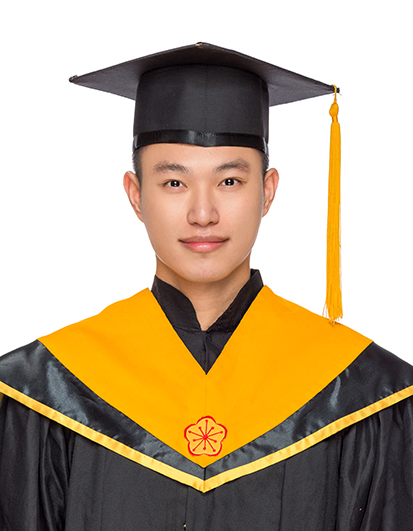
\includegraphics[width=0.5\textwidth]{picture/master_graduation_photo.jpeg} % Adjusted image size
    \end{minipage}
\end{tabularx}

\vspace{0.5cm}

\section*{Work Experience}
\begin{tabularx}{\textwidth}{Xr}
    \textbf{Research \& Development Engineer, ASUSTEK COMPUTER INC.} & \textit{2023--present} \\
\end{tabularx}
\begin{itemize}[leftmargin=30pt]
    \item \textbf{Production Scheduling Optimization System:}
    \begin{itemize}
        \item Utilized mathematical expertise to streamline the size of mathematical models, reducing execution time from over a day to within an hour.
        \item Adapted original models to meet specific production rules and requirements.
    \end{itemize}
    \item \textbf{GAI Recruiter System:}
    \begin{itemize}
        \item Implemented a sliding window approach to enable real-time speech recognition using the Whisper model.
        \item Reduced error rates by leveraging contextual information and fine-tuning parameters such as \texttt{vad\_filter} and \texttt{no\_repeat\_ngram\_size}.
    \end{itemize}
\end{itemize}

\section*{Education}
\begin{tabularx}{\textwidth}{Xr}
    \textbf{Master of Mathematics, NATIONAL TAIWAN UNIVERSITY} & \textit{2021--2023} \\
\end{tabularx}
\begin{itemize}[leftmargin=30pt]
    \item \textbf{Master's Thesis:} Introduction to the Ising Model and the Ising Model with Disorders:
    \begin{itemize}
        \item Applied probability methods to investigate disordered statistical physics models.
    \end{itemize}
    \item \textbf{Teaching Assistant:} Mathematical Analysis, Probability Theory.
    \item \textbf{Courses:}
    \begin{itemize}
        \item Data Structure and Algorithm, Machine Learning: Completed programming tasks using Python and C.
        \item Mathematics: Completed over 100 credits of math courses during undergraduate and master's studies.
    \end{itemize}
\end{itemize}

\noindent
\begin{tabularx}{\textwidth}{Xr}
    \textbf{Bachelor of Mathematics, NATIONAL TAIWAN UNIVERSITY} & \textit{2017--2021} \\
\end{tabularx}
\begin{itemize}[leftmargin=30pt]
    \item \textbf{NCTS Undergraduate Research Program:} Noncommutative Probability Theory:
    \begin{itemize}
        \item Participated in a study group hosted by the Quantum Computing Research Center of Hon Hai Research Institute (鴻海研究院).
    \end{itemize}
\end{itemize}

\noindent
\begin{tabularx}{\textwidth}{Xr}
    \textbf{Class of Science (科學班), TAIPEI MUNICIPAL CHIEN KUO HIGH SCHOOL} & \textit{2014--2017} \\
\end{tabularx}

\section*{Awards}
\begin{itemize}[leftmargin=30pt]
    \item NCTS Undergraduate Summer Research Program.
    \item Symposium for Young Analysts at National Central University.
    \item The Phi Tau Phi (斐陶斐) Scholastic Honor Society of the Republic of China Honorary Membership.
\end{itemize}

\section*{}
\begin{tabularx}{\textwidth}{X X}
    \textbf{Skills:} & \textbf{Hobbies:} \\
    Python, C++, Git, Linux, SQL, \LaTeX & Juggling \\
\end{tabularx}

\end{document}